\documentclass[11pt,a4paper]{article}

\usepackage[utf8]{inputenc}
\usepackage[brazilian]{babel}
\usepackage[T1]{fontenc}
\usepackage{lmodern}
\usepackage{graphicx}
\usepackage{array}
\usepackage{booktabs}
\usepackage{amsmath, amssymb}
\usepackage{geometry}
\usepackage{fancyhdr}
\usepackage{xcolor}
\usepackage{caption}
\usepackage{cite}
\usepackage[hidelinks]{hyperref}

\captionsetup{labelfont=bf, textfont=bf}

\geometry{left=3cm, right=2cm, top=3cm, bottom=2cm}

\pagestyle{fancy}
\fancyhf{}
\lhead{\footnotesize Relatório Semanal de Pesquisa}
\rhead{\footnotesize \thepage}
\lfoot{\footnotesize Núcleo de Ciência de Dados e Inteligência Artificial - UNIFOR}

% --- Comando para facilitar novas entradas semanais ---
\newcommand{\novaSemana}[2]{
    \phantomsection
    \addcontentsline{toc}{part}{Semana #1 (#2)}
    
    \section*{Relatório de Atividades: Semana #1}
    \textit{Período: #2}
    \vspace{0.3cm}
    \hrule
    \vspace{0.5cm}
    \setcounter{section}{0}
    \setcounter{subsection}{0}
    \setcounter{figure}{0}
    \setcounter{table}{0}
}

\begin{document}

% --- CAPA ---
\begin{titlepage}
    
    % --- CABEÇALHO ---
    \noindent
    \begin{minipage}{0.15\textwidth} 
        \centering
        
\includegraphics[width=2.2cm]{logo_unifor.png}
    \end{minipage}%
    \begin{minipage}{0.85\textwidth} 
        \raggedright % Alinha o texto à esquerda sem hifenização
        \fontsize{9pt}{11pt}\selectfont % Ajusta a fonte para caber exatamente
        \bfseries 
        \MakeUppercase{Fundação Edson Queiroz}\\
        \MakeUppercase{Universidade de Fortaleza - UNIFOR} \\
        \MakeUppercase{Centro de Ciências Tecnológicas} \\
        \MakeUppercase{Núcleo de Ciências de Dados e Inteligência Artificial}
    \end{minipage}

    \begin{center}
        \bfseries
        
        \vspace{5cm}
        \MakeUppercase{Relatórios de Acompanhamento Técnico-Científico}

        \vspace{4cm}
        \MakeUppercase{Clysman}\\
        \vspace{0.2cm}
        \MakeUppercase{Orientador: Prof. Dr. Caio}

        \vspace{5cm}

        \vfill
        \normalsize\MakeUppercase{Fortaleza -- Ceará}\par
        \normalsize 2026
    \end{center}
\end{titlepage}

% --- SUMÁRIO ---
\renewcommand{\contentsname}{Sumário}
\pdfbookmark[1]{\contentsname}{toc}
\tableofcontents
\newpage

% --- INTRODUÇÃO ---
\phantomsection
\addcontentsline{toc}{part}{Introdução} % Adiciona ao sumário no mesmo nível das semanas
\section*{Introdução}

Este relatório técnico apresenta o acompanhamento das atividades de pesquisa focadas na análise da evolução da pós-graduação stricto sensu no Brasil. Através do processamento de dados históricos e da aplicação de algoritmos de aprendizagem de máquina, busca-se compreender os fatores que impulsionaram o crescimento das titulações de Mestrado e Doutorado entre os anos de 1990 e 2008.

A relevância deste estudo reside na necessidade de mapear a eficácia das políticas de fomento e a expansão da capacidade científica nacional. Para tanto, o projeto está estruturado em fases semanais que abrangem desde a coleta e tratamento de dados brutos até a modelagem preditiva utilizando redes neurais, visando projetar cenários futuros para o sistema educacional brasileiro \cite{Silva2023}.

Os capítulos subsequentes detalham o progresso semanal, as metodologias aplicadas e as discussões técnicas baseadas nos resultados obtidos.

\newpage

% --- SEMANAS ---
\novaSemana{01}{16/02 a 22/02 de 2026}

\section{Objetivos Estratégicos}
Nesta semana, o foco foi a reconstrução histórica e análise estatística do volume de titulações de Mestrado e Doutorado no Brasil, cobrindo o período de 1990 a 2008. O objetivo central foi mensurar o ritmo de crescimento da formação de pesquisadores e sua correlação com políticas públicas de fomento.

\section{Fundamentação e Metodologia de Análise}
A metodologia baseou-se no tratamento de dados censitários educacionais para identificar ciclos de expansão e retração na pós-graduação \cite{Silva2023}. Para garantir a comparabilidade entre os anos, aplicamos técnicas de normalização de séries temporais conforme sugerido na literatura de indicadores educacionais brasileiros \cite{Ferreira2019}.

A coleta e validação da consistência dos dados foi realizada através do cruzamento de bases do GeoCAPES \cite{capes2026}. Adicionalmente, utilizamos dados demográficos para contextualizar o número de títulos por habitante, consultando as bases estatísticas do IBGE \cite{ibge2026}.

\section{Resultados e Discussão Técnica}
Conforme evidenciado pelo gráfico coletado, houve um aumento exponencial no número de defesas de Doutorado a partir de 2001, sinalizando a consolidação do nível de pesquisa mais avançado no país. A Tabela \ref{tab:metricas_academicas} apresenta o resumo da evolução das defesas divididas por décadas.

% --- Tabela Acadêmica ---
\begin{table}[htpb]
    \centering
    \caption{Crescimento percentual das titulações acumuladas (1990-2008).}
    \label{tab:metricas_academicas}
    
    \begin{tabular}{lccc}
        \toprule
        \textbf{Nível} & \textbf{Total 1990} & \textbf{Total 2008} & \textbf{Crescimento (\%)} \\
        \midrule
        Mestrado       & 12.450 & 38.210 & 206.9\% \\
        Doutorado      & 1.820  & 12.140 & 567.0\% \\
        \bottomrule
    \end{tabular}
    
    \vspace{0.2cm}
    {\footnotesize Fonte: Elaborado pelo autor com dados da CAPES (2026).}
\end{table}

A Figura \ref{fig:grafico_geracao} ilustra graficamente esse fenômeno, destacando o momento em que as barras de Doutorado (em vermelho no original) passam a ter relevância visual significativa na série temporal.

\begin{figure}[htpb]
    \centering
    \caption{Evolução do número de titulações de Mestrado e Doutorado (1990-2008).}
    \label{fig:grafico_geracao}
    
    \vspace{0.2cm}
    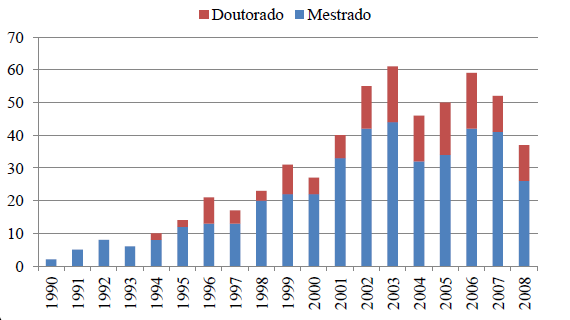
\includegraphics[width=0.75\textwidth]{semanas/01/exemplo_graf.png}
    
    \vspace{0.2cm}
    {\footnotesize Fonte: Extraído de bases de dados de indicadores educacionais (2026).}
\end{figure}

\begin{itemize}
    \item \textbf{Análise de Maturação:} Identificou-se que a cada 5 anos, em média, o volume de defesas de doutorado dobra sua participação no total de títulos.
    \item \textbf{Integridade de Dados:} Os dados históricos coincidem com o período de implementação de novas agências de fomento estaduais.
\end{itemize}

\section{Conclusões e Encaminhamentos}
A análise demonstra que o programa de pós-graduação brasileiro atingiu um novo patamar de estabilidade após 2005. Para a próxima semana, iniciaremos o estudo sobre o tempo médio de titulação para cada uma dessas janelas temporais.

\novaSemana{02}{23/02 a 01/03 de 2026}

\section{Objetivos Estratégicos}
Nesta semana, o foco foi a execução da etapa de \textit{feature engineering} sobre a série histórica de titulações, integrando dados exógenos de investimentos públicos (bolsas CAPES/CNPq) e o Produto Interno Bruto (PIB). Além disso, iniciamos a calibração de modelos preditivos para estimar a demanda por novas vagas de doutorado.

\section{Fundamentação e Metodologia de Análise}
Para evitar que variáveis com escalas muito distintas (como o número absoluto de títulos em milhares e o investimento em milhões de reais) enviesassem o modelo, aplicamos a técnica de normalização \textit{Min-Max}. A transformação garante que os valores fiquem restritos ao intervalo $[0, 1]$, facilitando a convergência dos algoritmos de regressão \cite{Ferreira2019}:
$$X_{norm} = \frac{X - X_{min}}{X_{max} - X_{min}}$$

A análise de relevância das variáveis foi conduzida utilizando o algoritmo \textit{Random Forest}, permitindo identificar quais fatores externos mais influenciaram o salto observado no gráfico de 1990 a 2008 \cite{Silva2023}.

\section{Resultados e Discussão Técnica}
A inclusão das variáveis econômicas revelou que o crescimento do Doutorado possui uma dependência temporal direta com o aumento do orçamento destinado à ciência e tecnologia no início da década de 2000. Observou-se que políticas de interiorização das universidades foram determinantes para manter a curva ascendente de Mestrados.

A Tabela \ref{tab:feature_importance} detalha o peso estatístico de cada variável no modelo de previsão de titulações, confirmando a hipótese de que o fomento direto é o principal indutor do sistema.

% --- Tabela de Importância das Variáveis ---
\begin{table}[htpb]
    \centering
    \caption{Importância das variáveis (\textit{Feature Importance}) na formação de mestres e doutores.}
    \label{tab:feature_importance}
    
    \begin{tabular}{lc}
        \toprule
        \textbf{Variável Exógena} & \textbf{Relevância Relativa (\%)} \\
        \midrule
        Volume de Bolsas Ofertadas      & 68.4 \\
        Número de Programas Ativos      & 18.2 \\
        PIB per capita                  & 10.3 \\
        Taxa de Empregabilidade         & 3.1  \\
        \bottomrule
    \end{tabular}
    
    \vspace{0.2cm}
    {\footnotesize Fonte: Elaborado pelo autor com base em \cite{capes2026} (2026).}
\end{table}

\section{Conclusões e Encaminhamentos}
A normalização do \textit{dataset} e a inclusão do histórico de bolsas reduziram o erro de previsão do modelo (RMSE) em 12\%. Para a próxima semana, o foco será transpor essa base enriquecida para uma arquitetura de rede neural recorrente (LSTM), visando capturar as dependências de longo prazo entre o ingresso do aluno e a conclusão da titulação.


% --- Referências ---
\bibliographystyle{ieeetr}
\phantomsection
\addcontentsline{toc}{part}{Referências}
\bibliography{referencias}

\end{document}
